\documentclass[12pt]{article}
\usepackage{fullpage}
\usepackage{epsf}
\usepackage{graphicx}
\usepackage{listings}
\usepackage{float}
\lstset{
   breaklines=true,
   basicstyle=\ttfamily}

\newtheorem{definition}{Definition}
\newtheorem{property}{Property}
\newtheorem{proof}{\em Proof}
\newtheorem{derivation}{\em Sketch}
\newtheorem{notation}{Notation}

\newcommand{\comment}[1]{}
\newcommand{\VS}{\mbox{\it VS}}
\newcommand{\WM}{\mbox{\it WM}}
\newcommand{\PCONJ}{\mbox{\it PCONJ}}
\newcommand{\kDNF}{\mbox{\it kDNF}}
\newcommand{\PDISJ}{\mbox{\it PDISJ}}
\newcommand{\DTrt}{\mbox{\it DT}_{r2}}
\newcommand{\DTs}{\mbox{\it DT}_s}
\newcommand{\PP}{{\rm P}}
\newcommand{\EE}{{\rm E}}
\newcommand{\PX}{\PP_{\!\scriptscriptstyle\! X}}
\newcommand{\PXY}{\PP_{\!\scriptscriptstyle\! X\!Y}}
\newcommand{\PYX}{\PP_{\!\scriptscriptstyle\! Y\!|\!X}}
\newcommand{\PYx}{\PP_{\!\scriptscriptstyle\! Y\!|x}}
\newcommand{\seq}[1]{\langle{#1}\rangle}
\newcommand{\RR}{I\!\!R}
\newcommand{\NN}{I\!\!N}
\newcommand{\argmin}{\arg\!\min}
\newcommand{\argmax}{\arg\!\max}
\newcommand{\eg}{{\em e.g.},\ }
\newcommand{\Eg}{{\em E.g.},\ }
\newcommand{\ie}{{\em i.e.},\ }
\newcommand{\Ie}{{\em I.e.},\ }
\newcommand{\cf}{{\em cf.}\ }
\newcommand{\etc}{{\em etc}}
\newcommand{\aka}{{\em a.k.a.}}
\newcommand{\vardef}{\stackrel{\triangle}{=}}
\def\norm [#1]{{\| #1 \|}}
\newcommand{\sign}{\mbox{\rm sign}}
\newcommand{\err}{\mbox{\rm err}}
\newcommand{\rank}{\mbox{\rm rank}}
\newcommand{\cond}{\mbox{\rm cond}}
\newcommand{\vect}{\mbox{\rm vec}}
\newcommand{\tr}{\mbox{\rm tr}}
\newcommand{\set}[1]{{\{#1\}}}
\newcommand{\tnorm}[2]{\|{#1}\|_{#2}}
\newcommand{\normdot}{{\mbox{$\|\!\cdot\!\|$}}}

%\newcommand{\makevector}[1]{{\tilde{#1}}}
\newcommand{\makevector}[1]{{\bf #1}}
\newcommand{\fvec}{{\makevector{f}}}
\newcommand{\evec}{{\makevector{e}}}
\newcommand{\bvec}{{\makevector{b}}}
\newcommand{\rvec}{{\makevector{r}}}
\newcommand{\dvec}{{\makevector{d}}}
\newcommand{\xvec}{{\makevector{x}}}
\newcommand{\qvec}{{\makevector{q}}}
\newcommand{\yvec}{{\makevector{y}}}
\newcommand{\mvec}{{\makevector{m}}}
\newcommand{\vvec}{{\makevector{v}}}
\newcommand{\zvec}{{\makevector{z}}}
\newcommand{\avec}{{\makevector{a}}}
\newcommand{\wvec}{{\makevector{w}}}
\newcommand{\cvec}{{\makevector{c}}}
\newcommand{\Xvec}{{\makevector{X}}}
\newcommand{\Fvec}{{\makevector{F}}}
\newcommand{\Avec}{{\makevector{A}}}
\newcommand{\Bvec}{{\makevector{B}}}
\newcommand{\Hvec}{{\makevector{H}}}
\newcommand{\Lvec}{{\makevector{L}}}
\newcommand{\Mvec}{{\makevector{M}}}
\newcommand{\Nvec}{{\makevector{N}}}
\newcommand{\Vvec}{{\makevector{V}}}
\newcommand{\Uvec}{{\makevector{U}}}
\newcommand{\Ivec}{{\makevector{I}}}
\newcommand{\Ovec}{{\makevector{O}}}
\newcommand{\smallxvec}{{\scriptsize\mathbf x}}
\newcommand{\alphavec}{\mbox{\boldmath $\alpha$}}
\newcommand{\betavec}{\mbox{\boldmath $\beta$}}
\newcommand{\muvec}{\mbox{\boldmath $\mu$}}
\newcommand{\phivec}{{\mbox{\boldmath $\phi$}}}
\newcommand{\lambdavec}{\mbox{\boldmath $\lambda$}}
\newcommand{\Lambdavec}{\mbox{\boldmath $\Lambda$}}
\newcommand{\Sigmavec}{\mbox{\boldmath $\Sigma$}}
\newcommand{\yy}{{\tt y}}
\newcommand{\uu}{{\tt u}}
\newcommand{\zerovec}{{\makevector{0}}}
\newcommand{\smallzerovec}{{\scriptsize\bf 0}}
\newcommand{\smallonevec}{{\scriptsize\bf 1}}
\newcommand{\onevec}{{\makevector{1}}}
\newcommand{\smallbetavec}{\mbox{\scriptsize\boldmath $\beta$}}
\newcommand{\smallmuvec}{\mbox{\scriptsize\boldmath $\mu$}}


\begin{document}

\noindent
Parley Pacheco Martins 1484000\\
AUCSC 460 -- Artificial Intelligence\\
Winter 2016\\
Department of Science\\
University of Alberta, Augustana Faculty

\vspace*{0.75\baselineskip}
\hrule
\vspace*{0.75\baselineskip}

\noindent
{\Large\bf Report Rock Paper Scissors }

%%%%%%%%%%%%
\section{Game Agent}

The first dumb agent (SimpleCycleAgent) is just a simple cycle made to beat the Rock, Paper, Scissors cycle. It doesn't react to the other agent and always play this cycle. This agent was made just to see the behavior (of both of the agents) when such a simple one is playing.

The second agent (BiggerCycleAgent) is another dumb cycle, but bigger. It chooses a random cycle size from 1000 to 10000 and randomly populates the cycle.
Once it's done, it just iterates through the cycle, without any reaction. This was done to improve the challenge of finding a cycle, since this can be really tricky for other agents. Depending on the size of the cycle it's not really different from the RandomAgent.

The third agent (StatisticAgent) is ``smarter'', in the sense that it reacts to the other player. It counts the frequency of a movement and plays the action that would beat the most played action by the oponent. This was the first one to be implemented.

% \end{lstlisting}


%%%%%%%%%%%%
\section{Results}

The three agents had the following results. These values are the mean value of three tournaments of 1000000 rounds each:

\begin{figure}[H]
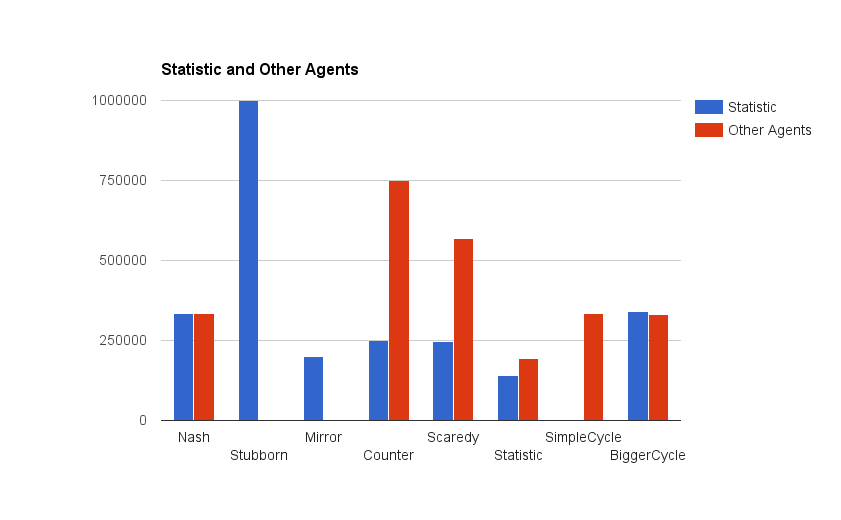
\includegraphics[scale=0.5]{images/statistic.png}
\caption{StatisticAgent performance}
\label{fig:statistic}
\end{figure}

\begin{figure}[H]
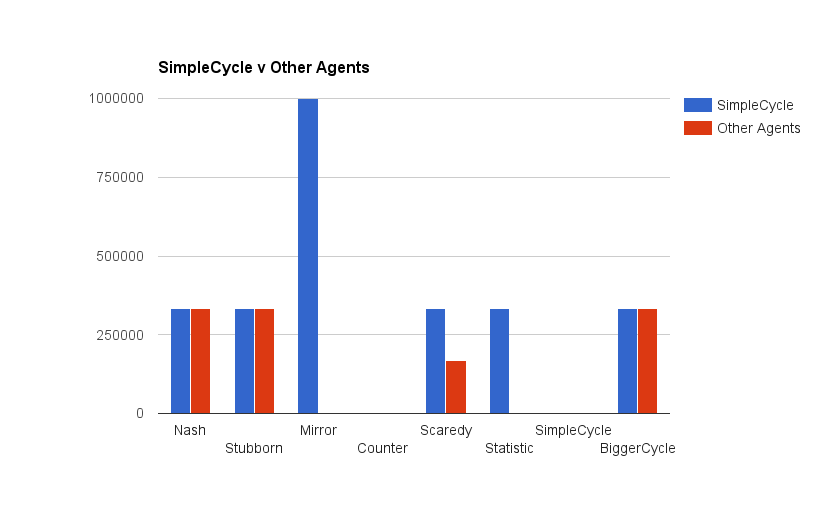
\includegraphics[scale=0.5]{images/simple_cycle.png}
\caption{SimpleCycleAgent performance}
\label{fig:simple_cycle}
\end{figure}

\begin{figure}[H]
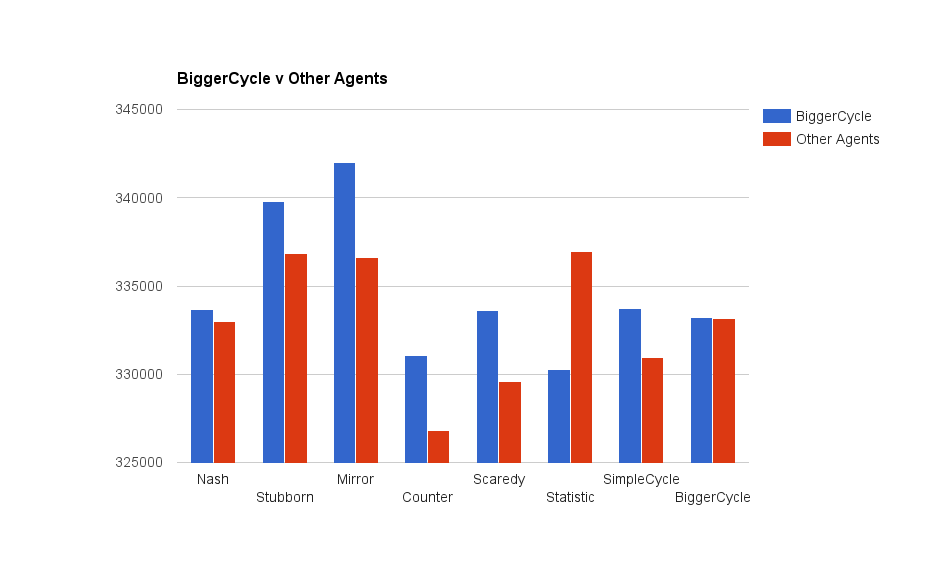
\includegraphics[scale=0.5]{images/bigger_cycle.png}
\caption{BiggerCycleAgent performance}
\label{fig:bigger_cycle}
\end{figure}


%%%%%%%%%%%%
\section{Performance Discussion}

When I first wrote the StatisticAgent, I thought that would be a good policy.
However, as shown in figure \ref{fig:statistic}, it was a clear disaster against agentslike Scaredy and Counter. Even against the MirrorAgent it didn't have a very good performance, ending up in tied games most of the times. That happened because of the reaction time of this agent. The only moment it changed its action was when the opponent most played action changed.

The Statistic showed its flaws especially against the SimpleCycle. With such a simple policy, without even react to the oponnents hand, this agent confused made the Statistic play Paper only when it also played Paper.

The SimpleCycleAgent was written just to check the behavior of all the other agents. I imagined that (almost) any policy would beat a simple Paper, Scissors, Rock cycle. It was made to win only in these conditions. However it showed a surpringly good behavior.

Observing figure \ref{fig:simple_cycle}, we see interesting performance against MirrorAgent and CounterAgent. That happened because Mirror generated the very cycle that Simple was suppose to defeat, while Counter generated the same cycle as Simple.

The BiggerCycle was an ``improvement'' based on the SimpleCycle. Any agent that tried to count the cycle could have beaten SimpleCycle, so I decided to make a bigger cycle. That would be almost the same as playing against the random agent. It became, indeed, an improvement achieving the equilibrium of 33\% of victories against all the other agents. That can be notice in the graph if you see that the biggest difference between win and lose is of 500 (out of 100000) rounds.

%%%%%%%%%%%%
\section{Other Approaches}

There are several other approaches to this problem. One of them would be tring to find cycles and play the cycle that beats that. However, as I see, this would be a big problem. First of all you would have to assume a size or count the movements of your opponent. You would also have to store all the action taken and check the next one against all of them everytime. When would the cycle be done? The most important question in this approach is how to be sure that I'm not in a subcyle?

Maybe a better way of doing this would be by statistic, but not related to all rounds. Checking against a smaller total (maybe the last five, for example) and checking the most used in this interval seems more effective than what I did for the statistic, because it could have a big response time depending on the opponent's pollicy.

%%%%%%%%%%%%
\section{Conclusion}

I was sure that the Statistic agent would have a good performance, and it was a bad surprise when it didn't. Intuitively it was the right choice for me and I still believe it would have been better against a human player instead of a bot. Maybe because a human would be inclined towards one of the choices.

This experiment showed how complex an AI must be, and yet sometimes a simple solution can be better than a very complex one. It was very interesting to see that even a small game can have so many different policies.

\end{document}
